% vim:autoindent:set textwidth=78:

\section{Comenzar}\label{label_getstarted}

% when the revision of a section has been finalized, 
% comment out the following line:
% \updatedisclaimer

Este capítulo ofrece un vistazo rápido de la instalación de QGIS, algunos datos disponibles 
en la página web de QGIS y cómo ejecutar una primera sesión sencilla
visualizando capas ráster y vectoriales.

\subsection{Instalación}\label{label_installation}
\index{installation}

La instalación de QGIS es muy sencilla. Hay disponibles paquetes de instalación estándar
para MS Windows y Mac OS X. Para muchos sabores de GNU/Linux se proporcionan paquetes
binarios (rpm y deb) o repositorios de software para añadir a su administrador
de instalación. Consiga la última información sobre paquetes binarios en la web de
QGIS en \url{http://qgis.osgeo.org/download/}.

Si necesita compilar QGIS a partir del código fuente, esto está documentado en el Apéndice
\ref{sec:install_windows} para MS Windows \win, Apéndice
\ref{sec:install_macosx} para Mac OSX \osx y Apéndice
\ref{sec:install_linux} para GNU/Linux \nix. Las instrucciones de instalación se
distribuyen con el código fuente de QGIS y también están disponibles en
\url{http://qgis.osgeo.org}.

\subsection{Datos de muestra}\label{label_sampledata}
\index{data!sample} 

La guía de usuario contiene ejemplos basados en el conjunto de datos
de muestra de QGIS.

\win El instalador de Windows tiene una opción para descargar los datos de muestra de QGIS.
Si se marca, los datos se descargarán en su carpeta \filename{Mis Documentos}
y se colocarán en una carpeta llamada \filename{GIS Database}. 
Puede usar el Explorador de Windows para mover esta carpeta a cualquier ubicación apropiada.
Si no seleccionó la casilla para instalar los datos de muestra
durante la instalación inicial de QGIS puede
\begin{itemize}
\item usar datos SIG que ya tenga;
\item descargar los datos de muestra de la web de QGIS
 \url{http://qgis.osgeo.org/download}; o
\item desinstalar QGIS y reinstalarto con la opción de descarga de datos marcada.
\end{itemize}

\nix \osx Para GNU/Linux y Mac OSX aún no hay disponibles paquetes de instalación 
del conjunto de datos en forma de rpm, deb o dmg. Para usar los datos de muestra
descargue el archivo \filename{qgis\_sample\_data} como archivo ZIP o TAR desde
\url{http://download.osgeo.org/qgis/data/} y descomprímalo en su equipo.
El conjunto de datos de Alaska incluye todos los datos SIG que se usan como
ejemplos y capturas de pantalla en la guía de usuario y también incluye una pequeña
base de datos de GRASS. La proyección de los datos de muestra de QGIS es Alaska Albers Equal
Area con unidades en pies. El código EPSG es 2964.

\begin{verbatim}
PROJCS["Albers Equal Area",
    GEOGCS["NAD27",
        DATUM["North_American_Datum_1927",
            SPHEROID["Clarke 1866",6378206.4,294.978698213898,
                AUTHORITY["EPSG","7008"]],
            TOWGS84[-3,142,183,0,0,0,0],
            AUTHORITY["EPSG","6267"]],
        PRIMEM["Greenwich",0,
            AUTHORITY["EPSG","8901"]],
        UNIT["degree",0.0174532925199433,
            AUTHORITY["EPSG","9108"]],
        AUTHORITY["EPSG","4267"]],
    PROJECTION["Albers_Conic_Equal_Area"],
    PARAMETER["standard_parallel_1",55],
    PARAMETER["standard_parallel_2",65],
    PARAMETER["latitude_of_center",50],
    PARAMETER["longitude_of_center",-154],
    PARAMETER["false_easting",0],
    PARAMETER["false_northing",0],
    UNIT["us_survey_feet",0.3048006096012192]]
\end{verbatim}

Si pretende usar QGIS como entorno gráfico para GRASS, puede encontrar una
selección de localizaciones de muestra (ej. Spearfish o Dakota del Sur) en la web
oficial de GRASS \url{http://grass.osgeo.org/download/data.php}.

\subsection{Sesión de ejemplo}\label{samplesession}

Ahora que tiene instalado QGIS y un conjunto de datos de muestra disponible, nos gustaría 
mostrarle una corta y sencilla sesión de ejemplo de QGIS. Visualizaremos una capa 
ráster y una vectorial. Usaremos la capa ráster de cobertura del terreno 
\filename{qgis\_sample\_data/raster/landcover.img} y la capa vectorial de lagos 
\filename{qgis\_sample\_data/gml/lakes.gml}.

\minisec{Iniciar QGIS}

\begin{itemize}
\item \nix{Arranque QGIS escribiendo: \usertext{qgis} en la línea de órdenes.}
\item \win{Arranque QGIS usando el menú Inicio o un acceso directo del escritorio, 
o haciendo doble clic en un archivo de proyecto de QGIS.}
\item \osx{Doble clic en el icono de su carpeta de Aplicaciones.}
\end{itemize} 

\minisec{Cargar capas ráster y vectoriales del conjunto de datos de muestra}

\begin{enumerate}
\item Haga clic en el icono \toolbtntwo{mActionAddRasterLayer}{Añadir capa ráster}.
\item Navegue a la carpeta \filename{qgis\_sample\_data/raster/}, seleccione el
archivo Img de ERDAS \filename{landcover.img} y pulse el botón \button{Abrir}.
\item Ahora pulse en el icono \toolbtntwo{mActionAddOgrLayer}{Añadir capa vectorial}.
\item Navegue a la carpeta \filename{qgis\_sample\_data/gml/}, seleccione
el archivo GML \filename{lakes.gml} y pulse el botón \button{Abrir}.
\item Acerque el zum un poco al área que prefiera con algunos lagos.
\item Haga doble clic en la capa \filename{lakes} en la leyenda del mapa para abrir el 
diálogo \dialog{Propiedades de la capa}.
\item Pulse en la pestaña \tab{Simbología} y seleccione un color de relleno azul.
\item Haga clic en la pestaña \tab{Etiquetas} y marque la casilla \checkbox{Mostrar etiquetas} 
para activar el etiquetado.
\item Pulse el botón \button{Aplicar}.
\end{enumerate} 

\begin{figure}[ht]
   \begin{center}
   \caption{Una sesión de QGIS sencilla \nixcaption}\label{fig:simple_session}\smallskip
   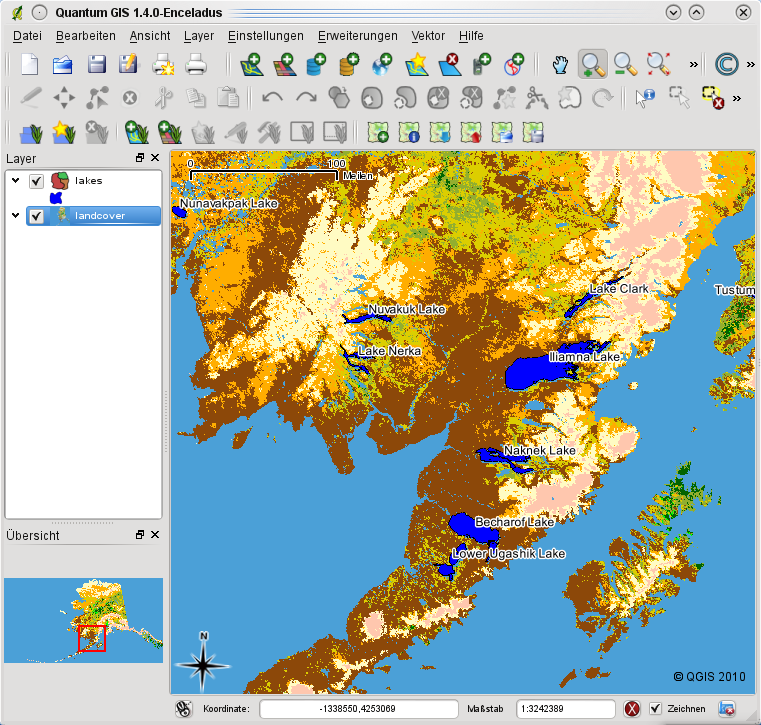
\includegraphics[clip=true, width=14cm]{simple_session}
\end{center}  
\end{figure}

Puede ver lo fácil que es visulizar capas ráster y vectoriales en 
QGIS. Vayamos a las secciones que siguen para aprender más sobre las 
funcionalidades disponibles, características y configuraciones y sobre cómo usarlas.
